%!TEX root = ../report.tex
\chapter{System Context}
\label{ch:context}

In this chapter the context of Docker is presented.%Improve 

\section{System Context}

%\subsection{History}
In this subsection an overview and global information about Docker project and history are presented. 

Docker is a open-source-software designed with the purpose of making the deployment of distributed application easier.
`Docker provides an integrated technology suite that enables development and IT operations teams to build, ship, and run distributed applications anywhere'\cite{whatisdocker}.

Docker helps to automate the deployment of applications inside so-called `containers' by making use of operating-system-level virtualization.

%borrowed from bsc thesis
Operating-system-level virtualization is a virtualization method where the kernel of an operating system allows the isolation of multiple instances of the user space of the operating system. Leveraging this type of virtualization over full virtualization (i.e. hardware emulation) offers a significant performance increase, because there is no need for emulation of the hardware.\cite{VirtualizationTechnologies}

\begin{figure}[b!]
\centering
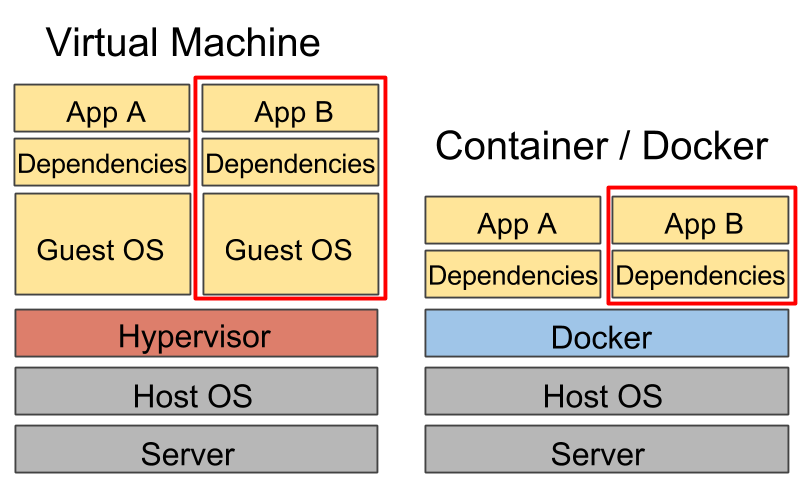
\includegraphics[scale=0.40,keepaspectratio=true]{./2-context/vmvsdocker}
\caption{Virtual machines compared to containers\cite{benchmarker}}
\label{fig:vmvsdocker}
\end{figure}

Figure \ref{fig:vmvsdocker} illustrates the difference between virtualization using hardware emulation and operating-system-level virtualization. As opposed to a virtual machine, a container does not have a guest operating system. Additionally, it does not need a hypervisor for emulating virtual hardware and trapping privileged instructions. This saves a lot of performance overhead. \\

One tool that makes use of operating-system-level virtualization is Docker. Docker can be used to package applications and dependencies in a `container'. Running this container using Docker will run it within a separate user space using operating-system-level virtualization. \\
Docker containers are instances of running Docker images. The process of creating a Docker image is relatively uncomplicated. It involves the creation of a so-called `Dockerfile', which is a type of Makefile, containing instructions that are to be executed to install the application and dependencies (using the \verb|RUN| instruction), and copy relevant data into the container (using \verb|ADD|). Every Dockerfile extends another image (using the \verb|FROM| instruction), which is either a previously created image or a base image (often containing the files of a specific operating system).

Docker images use a layered file system. Every command which is executed during the
build-process creates a new layer, where all modifications to the file system are stored.
Docker supports exporting images to tar-archives, which can be imported between similar versions of Docker.
%end of borrowed from bsc thesis

The first open-source version of Docker was released in March 2013. Docker is written in the Go Programming language \\


%\textit{https://en.wikipedia.org/wiki/Docker_\%28software\%29#History}

\section{Community}

% Always quote and reference https://www.docker.com/docker-community

In this subsection the developpers programming docker and the community around them are presented. \\
The creator of Docker is Solomon Hykes. \\

Docker started as an internal project within dotCloud, a platform-as-a-service company with four main developers. \\
The following organizations are the main contributors to Docker: the Docker team, Red Hat, IBM, Google, Cisco Systems and Amadeus IT Group. 

Docker has an active community and the managers encourage developpers around the world to contribute. 
\textit{https://docs.docker.com/opensource/project/who-written-for/}

There are several ways to get in contact with the community of Docker:
\begin{itemize}
\item IRC -- Here, the most knowledgeable Docker users reside. At the \verb|#docker| and \verb|#docker-dev| groups on \verb|irc.freenode.net|.

\item Google Groups -- The developers are active in the \verb|docker-dev| Google group.

\item Stack Overflow -- Questions about Docker itself can be asked on the Stack Overflow. 

\end{itemize}

